\documentclass[a4paper,10pt]{article}

\usepackage[brazilian]{babel}
\usepackage[left=2.5cm,right=2.5cm,top=3cm,bottom=2.5cm]{geometry}
\usepackage{mathtools}
\usepackage{amsthm}
\usepackage{amsmath}
%\usepackage{nccmath}
\usepackage{amssymb}
\usepackage{amsfonts}
\usepackage{physics}
%\usepackage{dsfont}
%\usepackage{mathrsfs}

\usepackage{titling}
\usepackage{indentfirst}

\usepackage{bm}
\usepackage[dvipsnames]{xcolor}
\usepackage{cancel}

\usepackage{xurl}
\usepackage[colorlinks=true]{hyperref}

\usepackage{float}
\usepackage{graphicx}
%\usepackage{tikz}
\usepackage{caption}
\usepackage{subcaption}

%%%%%%%%%%%%%%%%%%%%%%%%%%%%%%%%%%%%%%%%%%%%%%%%%%%

\newcommand{\eps}{\epsilon}
\newcommand{\vphi}{\varphi}
\newcommand{\cte}{\text{cte}}

\newcommand{\N}{\mathbb{N}}
\newcommand{\Z}{\mathbb{Z}}
\newcommand{\Q}{\mathbb{Q}}
\newcommand{\R}{\vb{R}}
\newcommand{\C}{\mathbb{C}}
\renewcommand{\S}{\hat{S}}
%\renewcommand{\H}{\s{H}}

\renewcommand{\a}{\vb{a}}
\newcommand{\nn}{\hat{n}}
\renewcommand{\d}{\dagger}
\newcommand{\up}{\uparrow}
\newcommand{\down}{\downarrow}

\newcommand{\0}{\vb{0}}
%\newcommand{\1}{\mathds{1}}
\newcommand{\E}{\vb{E}}
\newcommand{\B}{\vb{B}}
\renewcommand{\v}{\vb{v}}
\renewcommand{\r}{\vb{r}}
\renewcommand{\k}{\vb{k}}
\newcommand{\p}{\vb{p}}
\newcommand{\q}{\vb{q}}
\newcommand{\F}{\vb{F}}

\newcommand{\s}{\sigma}
%\newcommand{\prodint}[2]{\left\langle #1 , #2 \right\rangle}
\newcommand{\cc}[1]{\overline{#1}}
\newcommand{\Eval}[3]{\eval{\left( #1 \right)}_{#2}^{#3}}

\newcommand{\unit}[1]{\; \mathrm{#1}}

\newcommand{\n}{\medskip}
\newcommand{\e}{\quad \mathrm{e} \quad}
\newcommand{\ou}{\quad \mathrm{ou} \quad}
\newcommand{\virg}{\, , \;}
\newcommand{\ptodo}{\forall \,}
\renewcommand{\implies}{\; \Rightarrow \;}
%\newcommand{\eqname}[1]{\tag*{#1}} % Tag equation with name

\setlength{\droptitle}{-7em}

\theoremstyle{plain}
\newtheorem{theorem}{Teorema}[section]
%\newtheorem{defi}[theorem]{Definição}
\newtheorem{lemma}[theorem]{Lema}
%\newtheorem{corol}[theorem]{Corolário}
%\newtheorem{prop}[theorem]{Proposição}
%\newtheorem{example}{Exemplo}
%
%\newtheorem{inneraxiom}{Axioma}
%\newenvironment{axioma}[1]
%  {\renewcommand\theinneraxiom{#1}\inneraxiom}
%  {\endinneraxiom}
%
%\newtheorem{innerpostulado}{Postulado}
%\newenvironment{postulado}[1]
%  {\renewcommand\theinnerpostulado{#1}\innerpostulado}
%  {\endinnerpostulado}
%
%\newtheorem{innerexercise}{Exercício}
%\newenvironment{exercise}[1]
%  {\renewcommand\theinnerexercise{#1}\innerexercise}
%  {\endinnerexercise}
%
%\newtheorem{innerthm}{Teorema}
%\newenvironment{teorema}[1]
%  {\renewcommand\theinnerthm{#1}\innerthm}
%  {\endinnerthm}
%
\newtheorem{innerlema}{Lema}
\newenvironment{lema}[1]
  {\renewcommand\theinnerlema{#1}\innerlema}
  {\endinnerlema}
%
%\theoremstyle{remark}
%\newtheorem*{hint}{Dica}
%\newtheorem*{notation}{Notação}
%\newtheorem*{obs}{Observação}


\title{\Huge{\textbf{Lista 3 - Mecânica Estatística}}}
\author{Mateus Marques}

\begin{document}

\maketitle

\section*{2) Entropia para bósons e férmions}

Primeiramente, definamos o parâmetro $\zeta = \pm 1$, sendo $\zeta = +1$ referindo à bósons e $\zeta = -1$ a férmions. Queremos mostrar que
\begin{equation} \label{eq:entropia_ruim}
S = \zeta k_B \sum_{j} \Big[
(1 + \zeta n_j) \log(1 + \zeta n_j) - \zeta n_j \log n_j
\Big], \quad n_j = \frac{1}{e^{\beta(\eps_j-\mu)} - \zeta}.
\end{equation}
Desenvolvendo essa expressão (usando que $\zeta^2 = 1$), temos
$$
S = k_B \sum_{j} \qty[
\zeta \log(1 + \zeta n_j) +
n_j \log(\frac{1}{n_j} + \zeta)
].
$$
Substituindo a expressão de $n_j$ explícita:
$$
\zeta \log(1 + \zeta n_j) =
\zeta \log\qty[\frac{(e^{\beta(\eps_j-\mu)}-\cancel{\zeta})+\cancel{\zeta}}{e^{\beta(\eps_j-\mu)}-\zeta}] =
\zeta \qty{ \beta(\eps_j-\mu) + \log\qty[\frac{1}{e^{\beta(\eps_j-\mu)}-\zeta}] }.
$$
$$
n_j \log(\frac{1}{n_j} + \zeta) = \frac{1}{e^{\beta(\eps_j-\mu)}-\zeta}
\log[(e^{\beta(\eps_j-\mu)}-\cancel{\zeta})+\cancel{\zeta}] =
\frac{\beta (\eps_j-\mu)}{e^{\beta(\eps_j-\mu)}-\zeta}.
$$

A entropia então se simplifica para
$$
S = k_B \sum_{j}
\qty{
\zeta\log\qty[\frac{1}{e^{\beta(\eps_j-\mu)}-\zeta}] +
\beta(\eps_j-\mu) \qty[\frac{\zeta e^{\beta(\eps_j-\mu)}-\cancel{\zeta^2}+\cancel{1}}{e^{\beta(\eps_j-\mu)}-\zeta}] =
}
$$
\begin{equation} \label{eq:entropia_boa}
\boxed{ S = \zeta k_B \sum_{j}
\qty[
\log n_j +
\beta(\eps_j-\mu) e^{\beta(\eps_j-\mu)} n_j
]. }
\end{equation}

Dessa forma, temos que a equação \ref{eq:entropia_boa} é equivalente à equação \ref{eq:entropia_ruim}. Mostrarei que a entropia dos gases quânticos se escreve como na forma da equação \ref{eq:entropia_boa}.

\n

Como vimos em aula, no ensemble grande canônico a função de partição é
$$
Z = \prod_j Z_j, \quad Z_j = [1 \mp e^{-\beta(\eps_j-\mu)}]^{\mp 1}= [1 - \zeta e^{-\beta(\eps_j-\mu)}]^{-\zeta},
$$
onde $Z_j$ é a função de partição para o estado $j$. Perceba que $Z_j$ se reescreve como
$$
Z_j = \qty[\frac{1}{ 1 - \zeta e^{-\beta(\eps_j-\mu)} }]^{\zeta} =
\qty[\frac{e^{\beta(\eps_j-\mu)}}{ e^{\beta(\eps_j-\mu)} - \zeta }]^{\zeta} =
\Big[
e^{\beta(\eps_j-\mu)} n_j
\Big]^{\zeta}.
$$

Portanto, a entropia $S = -\pdvc{F}{T}{V,\mu}$, com $F = -k_B T \log Z$, é dada por
$$
S = \pdv{T} \qty(k_B T \sum_{j} \zeta \Big[\beta(\eps_j-\mu) + \log n_j\Big])_{V,\mu} =
$$
$$
= \zeta k_B \sum_{j} \Big[\cancel{\beta(\eps_j-\mu)} + \log n_j\Big] +
\zeta k_B \sum_{j} \qty{-\cancel{\beta (\eps_j - \mu)} + \beta(\eps_j-\mu) n_j e^{\beta(\eps_j-\mu)}} =
$$
$$
= \zeta k_B \sum_{j} \qty[\log n_j + \beta (\eps_j - \mu) n_j e^{\beta(\eps_j-\mu)}],
$$
que é exatamente a equação \ref{eq:entropia_boa}. Na dedução acima eu utilizei (mas não explicitei) as derivadas $T \pdv{\beta}{T} = -\beta$ e $T \pdv{\log n_j}{T} = \beta (\eps_j-\mu) n_j e^{\beta(\eps_j-\mu)}$. Isso termina o exercício.

\pagebreak

\section*{3) Radiação de corpo negro}

Um estado de partícula única é caracterizada pelo vetor de onda $\k$ e pela polarização $p$ do fóton. Sendo $E(\k) = \hbar c \abs{\k}$ a relação de dispersão, a DOS desse sistema é
$$
D(\eps) = \sum_{\k,p} \delta(\eps-E(\k)) = \frac{2V}{(2\pi)^3} \int \dd[3]{\k} \delta(\eps-E(\k)) =
\frac{V}{\pi^2} \int \dd{k} k^2 \delta(\eps-\underbrace{\hbar c k}_{x})
$$
$$
D(\eps) = \frac{V}{\pi^2 (\hbar c)^3} \int \dd{x} x^2 \delta(\eps-x)
= \frac{V \eps^2}{\pi^2 (\hbar c)^3}.
$$

Sendo $n(\eps)$ a distribuição de Bose-Einstein, como $E/V = \frac{1}{V} \int \eps D(\eps) n(\eps) \dd{\eps} = \int \hbar \omega \frac{D(\hbar\omega)}{V} \, n(\hbar\omega) \hbar \dd{\omega} = \int u(\omega) \dd{\omega}$, temos que a densidade de energia dos fótons com frequência entre $\omega$ e $\omega + \dd{\omega}$ é
$$
u(\omega) = \frac{1}{V} \hbar^2 \omega D(\hbar\omega) n(\hbar\omega) = \frac{\hbar^2 \omega \, \hbar^2 \omega^2}{\pi^2 \hbar^3 c^3} \cdot
\frac{1}{e^{\beta\hbar\omega} - 1} \implies
\boxed{ u(\omega) =
\frac{\hbar}{\pi^2 c^3} \cdot \frac{\omega^3}{e^{\beta\hbar\omega} - 1}. }
$$

A partir de $\abs{u(\omega) \dd{\omega}} = \abs{u(\lambda) \dd{\lambda}}$ e usando $h = 2\pi \hbar$, temos que
$$
u(\lambda) = u(\omega) \abs{\dv{\omega}{\lambda}} = u\qty(\frac{2\pi c}{\lambda}) \cdot \frac{2\pi c}{\lambda^2} \implies
\boxed{ u(\lambda) =
\frac{8 \pi h c}{\lambda^5} \cdot \frac{1}{e^{\beta hc / \lambda} - 1}. }
$$

\begin{figure}[H]
\centering
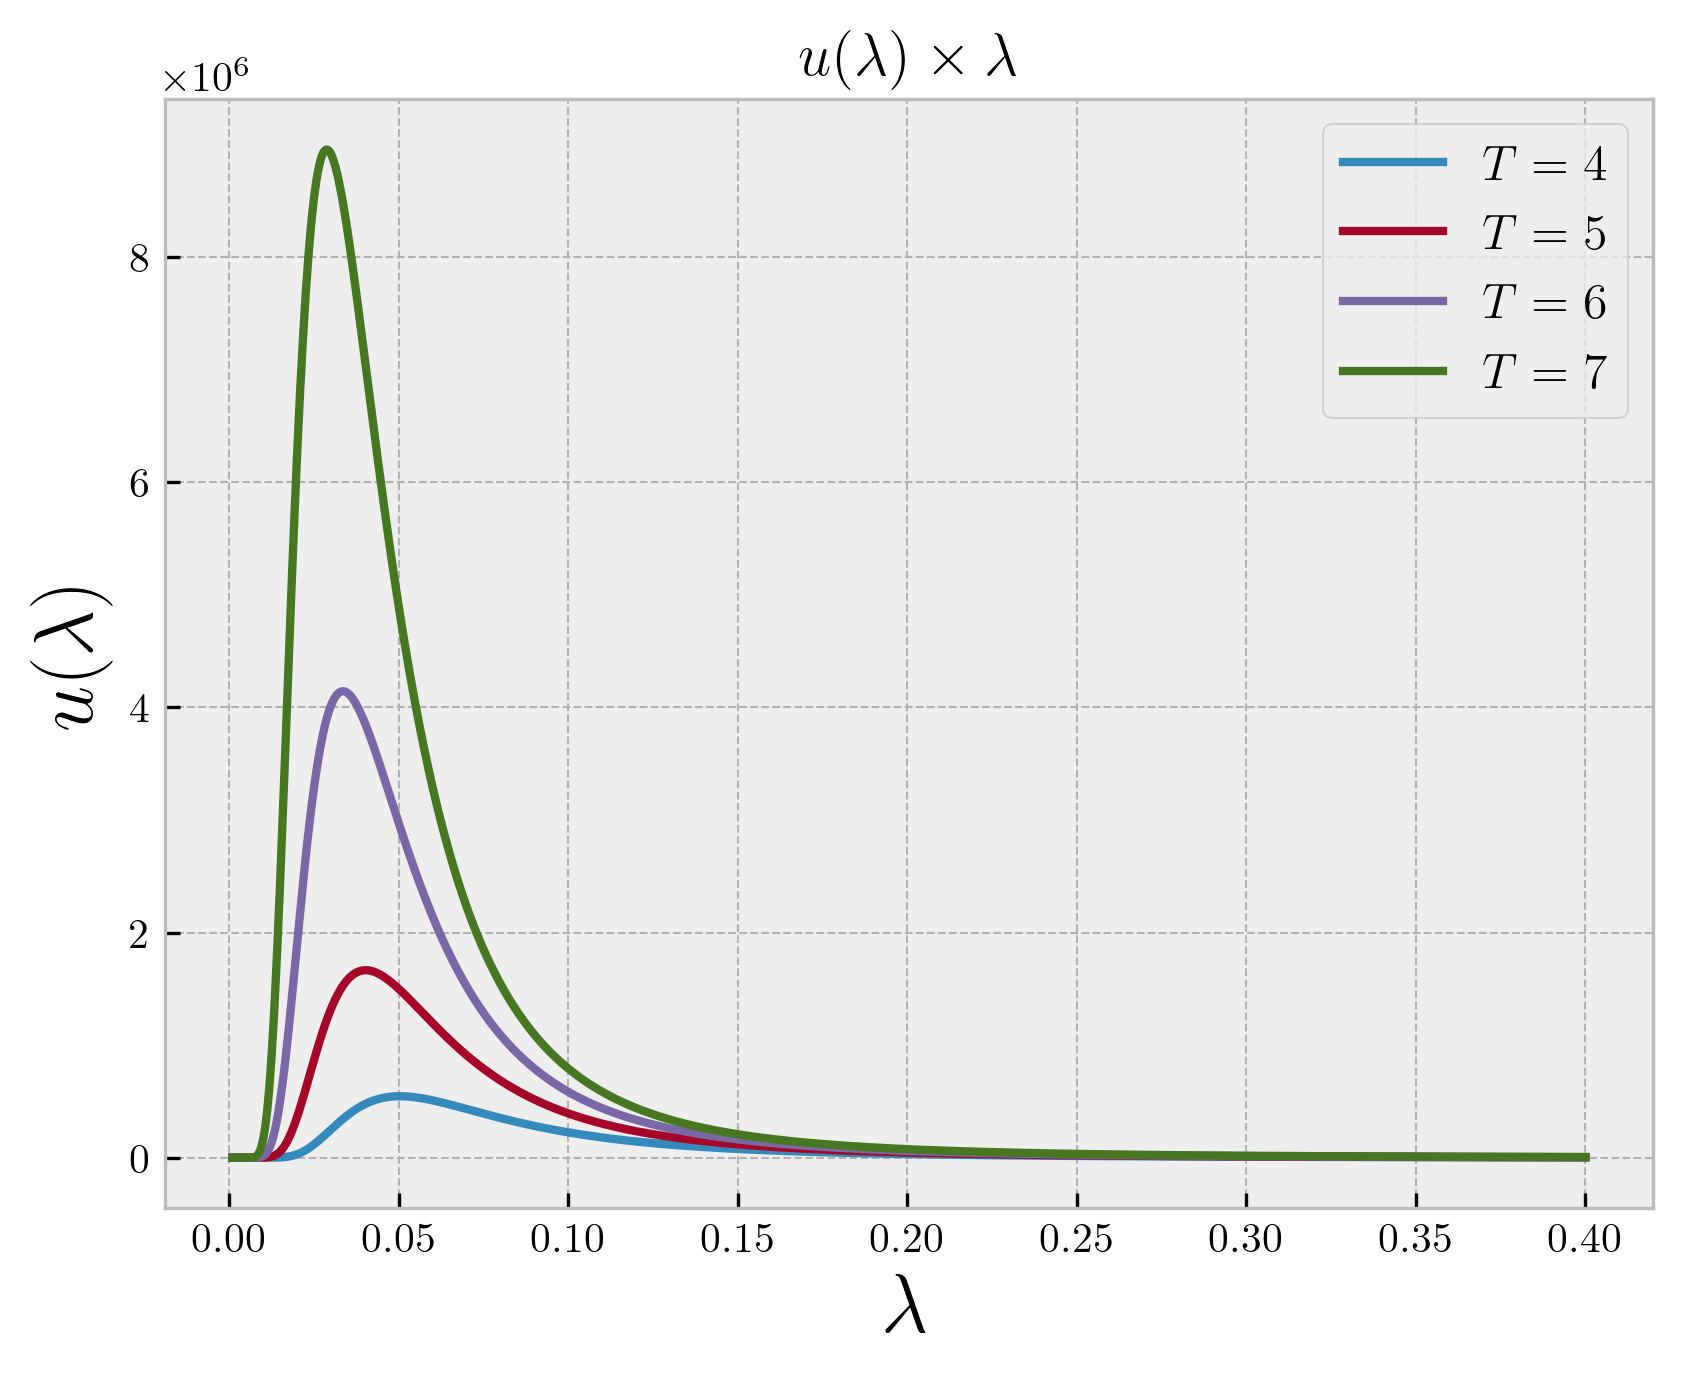
\includegraphics[width=0.6\linewidth]{fig/planck-lambda.png}
\caption{Distribuição $u(\lambda) \times \lambda$ para diferentes temperaturas em unidades arbitrárias $h = k_B = c = 1$.}
\label{fig:planck}
\end{figure}

A frequência $\omega$ correspondente ao máximo de $u(\omega)$ é obtida resolvendo $\dv{u(\omega)}{\omega} = 0$.
$$
\dv{u(\omega)}{\omega} =
\frac{\hbar \omega^2}{\pi^2 c^3 (e^{\beta\hbar\omega} - 1)}
\qty[3 - \beta\hbar\omega \frac{e^{\beta\hbar\omega}}{e^{\beta\hbar\omega} - 1}] =
$$
$$
=
\frac{3 \hbar \omega^2}{\pi^2 c^3 (e^{\beta\hbar\omega} - 1)^2}
\qty[e^{\beta\hbar\omega} \qty(1 - \frac{\beta\hbar\omega}{3}) - 1] = 0.
$$

Definindo $x = \beta\hbar\omega$, basta então que o Mathematica resolva a equação transcendente $x + 3e^{-x} = 3$. Ele retorna duas soluções $x_1 = 0$ e $x_2 \approx 2.82144$. Claramente o máximo está associado à solução $x_2$, de maneira que $\boxed{\omega_{\text{max}} = \frac{2.82144}{\beta\hbar}}$. Repare que essa é essencialmente a Lei de Wien, onde $\lambda_{\text{max}} T = \cte$.

\n

No limite $\hbar\omega \ll k_B T$, temos que $\beta \hbar \omega \to 0$ de maneira que $e^{\beta\hbar\omega} - 1 \approx \beta\hbar\omega$. Com isso temos que
$$
u(\omega) \approx \frac{\cancel{\hbar}}{\pi^2 c^3} \cdot \frac{\omega^3}{\beta\cancel{\hbar}\omega} = \frac{k_B T}{\pi^2 c^3} \omega^2,
$$
que é a distribuição clássica de Rayleigh-Jeans (RJ). Essa distribuição que gera a ``catástrofe do ultravioleta'', pois $u(\omega)$ cresce ilimitadamente com a frequência $\omega \to \infty$ (indo para o ultravioleta). Em particular, para a distribuição de Rayleigh-Jeans a energia emitida por um corpo negro a qualquer temperatura é infinita
$$
\frac{E}{V} = \int u_{\text{RJ}}(\omega) \dd{\omega} = +\infty,
$$
o que não faz sentido físico.

\n\n

(b) Com a mudança de variável $x = \beta \hbar\omega$, temos
$$
\frac{E}{V} = \int_0^\infty u(\omega) \dd{\omega} = \frac{\hbar}{\pi^2 c^3} \,
\qty(\frac{1}{\beta\hbar})^4 \int_0^\infty \frac{x^3}{e^{x} - 1} \dd{x}.
$$

Pedindo para o Mathematica calcular a integral acima, ele retorna $\int_0^\infty \frac{x^3}{e^{x} - 1} \dd{x} = \frac{\pi^4}{15}$. Portanto
$$
\frac{E}{V} = \frac{k_B^4 T^4}{\pi^2 \hbar^3 c^3} \cdot \frac{\pi^4}{15} =
\frac{4}{c} \, \underbrace{\qty(\frac{\pi^2 k_B^4}{60 \hbar^3 c^2})}_{\sigma} \, T^4 = \frac{4}{c} \sigma T^4.
$$

Temos $C_V = \pdvc{E}{T}{V,N} = \frac{16}{c} V \sigma T^3 \propto T^3$. O número de fótons é dado por ($x = \beta \eps$)
$$
\frac{N}{V} = \frac{1}{V} \int D(\eps) n(\eps) \dd{\eps} =
\frac{1}{\pi^2 (\hbar c)^3} \int_0^{\infty} \frac{\eps^2}{e^{\beta \eps}-1} \dd{\eps} =
\frac{1}{\pi^2 (\hbar c)^3} \cdot \frac{1}{\beta^3} \int_0^\infty \frac{x^2}{e^x - 1} \dd{x}.
$$

O Mathematica retorna $\int_0^\infty \frac{x^2}{e^x - 1} \dd{x} = 2 \zeta(3) \approx 2.40411$. Portanto
$$
\frac{N}{V} = \frac{2 \zeta(3) k_B^3}{\pi^2 \hbar^3 c^3} \cdot T^3,
$$
ou seja, o número de fótons é proporcional a $T^3$.

\n\n

(c) Como visto em aula, temos para fótons $\mu = 0$ e que o potencial termodinâmico de bósons é (usando o limite do contínuo $\sum_{\k,p} = \int \dd{\eps} D(\eps)$)
$$
\Phi = k_B T \sum_{\k,p} \log(1 - e^{-\beta (\eps_{\k} - \mu)}) = k_B T \int_0^{\infty} \dd{\eps} D(\eps) \log(1 - e^{-\beta \eps})
$$
$$
\Phi = \frac{V k_B T}{\pi^2 (\hbar c)^3} \int_0^{\infty} \eps^2 \log(1 - e^{-\beta \eps}) \dd{\eps} =
$$

A integral acima foi realizada no Mathematica e ele retornou $\int_0^{\infty} \eps^2 \log(1 - e^{-\beta \eps}) \dd{\eps} = - \frac{\pi^4}{45 \beta^3}$. Dessa maneira, obtemos
$$
\Phi = -\frac{V \pi^2 (k_B T)^4}{45 (\hbar c)^3} =
- \frac{4 V}{3 c} \cdot \underbrace{\qty(\frac{\pi^2 k_B^4}{60 \hbar^3 c^2})}_{\sigma} T^4 =
- \frac{V}{3} \underbrace{\qty(\frac{4}{c} \sigma T^4)}_{E} = -\frac{E V}{3}.
$$

Lembrando que $\Phi = - PV$, obtemos que
$$
\boxed{ P = \frac{1}{3} E. }
$$

\n\n

(d) Como vemos na Figura \ref{fig:cosmic}, o espectro da radiação cósmica de fundo é muito bem descrito pela curva $u(\lambda)$ do corpo negro. Uma possível explicação para essa ótima compatibilidade está contida no próprio modelo do Big Bang. Muito antes da formação de galáxias, o universo no começo era constituído de um plasma interagente, sendo bem menor e muito quente. Mas com a expansão do universo e seu resfriamento adiabático, tornou-se favorável a formação de átomos de hidrogênio eletricamente neutros, onde a temperatura média era em torno de 3000 K, segundo a \href{https://en.wikipedia.org/wiki/Cosmic_microwave_background}{Wikipédia}. A radiação cósmica de fundo que detectamos hoje foi originada de fótons emitidos a partir desse período, onde a temperatura era alta e o universo tinha um comportamento bem descrito por um corpo negro. Como os fótons interagiam fracamente com os átomos eletricamente neutros, eles puderam viajar livremente pelo espaço. A expansão do universo leva então a um red-shift no comprimento de onda dos fótons, que diminui suas energias e efetivamente faz com que o espectro de corpo negro tenha menor temperatura, a saber $T = 2.725 \unit{K}$.

\begin{figure}[H]
\centering
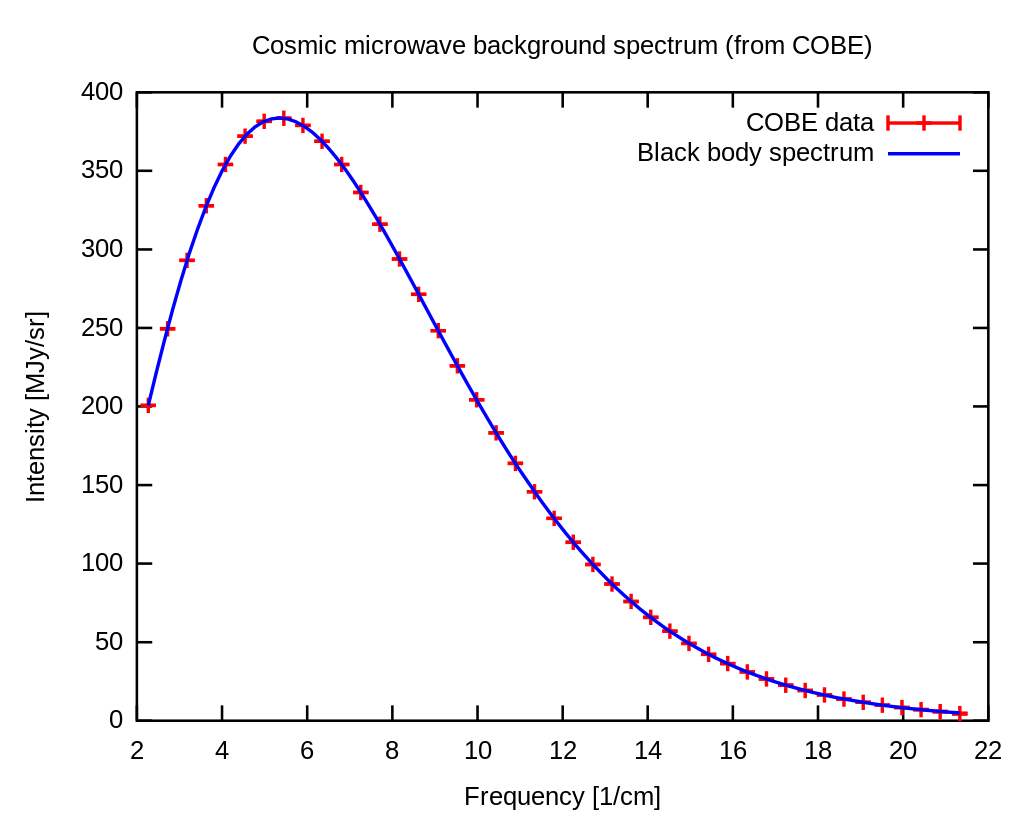
\includegraphics[width=0.6\linewidth]{fig/cosmic_bg.png}
\caption{Comparação do espectro da radiação cósmica de fundo com o espectro de corpo negro para $T = 2.725 \unit{K}$. Figura da \href{https://en.wikipedia.org/wiki/Cosmic_microwave_background}{Wikipédia}.}
\label{fig:cosmic}
\end{figure}


\pagebreak

\section*{5) Condensado de Bose-Einstein: duas dimensões e armadilha parabólica}

(a) Calculemos a DOS para o gás de bósons livres em duas dimensões (com dispersão $\eps = \hbar^2 k^2 / 2m$, temos que
$k = \sqrt{2m\eps/\hbar^2}$ e $\dd{k} = \sqrt{\frac{m}{2\hbar^2\eps}} \dd{\eps}$):
$$
\sum_{\k, \sigma} = \frac{g V}{(2\pi)^2} \int \dd[2] k = \frac{gV}{2\pi} \int \dd{k} k =
\frac{gV}{2\pi} \int \sqrt{\frac{m}{2\hbar^2\eps}} \dd{\eps} \sqrt{2m\eps/\hbar^2} =
$$
$$
= \int \dd{\eps} \frac{mgV}{2\pi \hbar^2} = \int \dd{\eps} D(\eps),
$$
onde obtemos $D(\eps) = \frac{mgV}{2\pi \hbar^2}$ em duas dimensões.

\n

Substituindo $x = \beta \eps$, temos
$$
N = \int D(E) n(E) \dd{E} = \frac{m g V}{2\pi \hbar^2} \int_0^{\infty} \frac{1}{e^{\beta (\eps-\mu)} - 1} \dd{\eps} =
k_B T \cdot \frac{m g V}{2\pi \hbar^2} \int_0^{\infty} \frac{1}{e^{(x - \beta\mu)} - 1} \dd{x}.
$$

\n

Para $T > T_c$ temos que $\mu < 0$, e que $\mu \to 0^-$ quando $T \to T_c$. Isso nos dá que
$$
\frac{N}{V} = T_c \, \frac{k_B m g V}{2\pi \hbar^2} \int_0^{\infty} \frac{1}{e^{x} - 1} \dd{x},
$$
só que a integral $\int_0^{\infty} \frac{1}{e^{x} - 1} \dd{x} = +\infty$ é divergente no infravermelho (para $x \to 0^+$). Isso implica que $\boxed{T_c = 0}$ para o condensado de Bose-Einstein livre em duas dimensões.

\n

(b) Para o gás de bósons em uma armadilha parabólica, a hamiltoniana do sistema é
$$
H = \qty(\frac{\hat{P}_x^2}{2m} + \frac{m \omega_x^2}{2} \hat{X}^2) +
\qty(\frac{\hat{P}_y^2}{2m} + \frac{m \omega_y^2}{2} \hat{Y}^2) +
\qty(\frac{\hat{P}_z^2}{2m} + \frac{m \omega_z^2}{2} \hat{Z}^2),
$$
que é um oscilador harmônico em 3D. Como sabemos, as autoenergias do oscilador harmônico em 1D são $E_n = \hbar\omega(n+\frac{1}{2})$. Então para o oscilador 3D é a soma $E_{n_x, n_y, n_z} = \frac{\hbar}{2} (\omega_x + \omega_y + \omega_z) + \hbar(\omega_x n_x + \omega_y n_y + \omega_z n_z)$. Para o oscilador harmônico 1D, também sabemos que as autofunções são dadas por polinômios de Hermite
$$
\psi_n(x) = \frac{1}{\sqrt{2^n n!}} \qty(\frac{m\omega}{\pi\hbar})^{1/4} e^{-\frac{m\omega x^2}{2\hbar}}
H_n\qty(\sqrt{\frac{m\omega}{\hbar}} x).
$$

Em particular, no estado fundamental $n = 0$ temos $\psi_0(x) = \qty(\frac{m\omega}{\pi\hbar})^{1/4} e^{-\frac{m\omega x^2}{2\hbar}}$. Como o oscilador harmônico 3D é o produto tensorial de três osciladores 1D, a função de onda do estado fundamental é o produto dos estados fundamentais dos três osciladores 1D
$$
\Psi_0(x,y,z) =
\qty(\frac{m}{\pi\hbar})^{3/4}
(\omega_x \omega_y \omega_z)^{1/4}
\exp[-\frac{m}{2\hbar} (\omega_x x^2 + \omega_y y^2 + \omega_z z^2)].
$$

\n

Como o condensado é um sistema de bósons (não há restrições na ocupação dos estados), no limite termodinâmico $N \to \infty$ e à temperatura baixa, o estado $\ket{\Psi_0}$ é macroscopicamente ocupado. Devido à interpretação estatística da função de onda, se o número de partículas num estado $\ket{\Psi}$ é muito grande, medir o módulo quadrado $\abs{\Psi(\r)}^2$ (ao redor do ponto $\r$) corresponde a medir a densidade de partículas no ponto $\r$ (com volume infinitesimal $\dd[3]{\r}$), dado que usemos uma normalização $\int \abs{\Psi(\r)}^2 \dd[3]{\r} = N$. Com isso podemos interpretar que a densidade de partículas é dada por $n(\r) = \abs{\Psi(\r)}^2$.

\n

Para a armadilha parabólica, a densidade de partículas no estado fundamental é
$$
n(\r) = N \abs{\Psi_0(x,y,z)}^2 =
N\qty(\frac{m}{\pi\hbar})^{3/2}
(\omega_x \omega_y \omega_z)^{1/2}
\exp[-\frac{m}{\hbar} (\omega_x x^2 + \omega_y y^2 + \omega_z z^2)].
$$

\n

Para estimar o volume do condensado, analisaremos a região do espaço que as partículas no estado fundamental podem ocupar. Por exemplo, para a coordenada $x$ a parte correspondente da hamiltoniana é $H_x = \frac{p_x^2}{2m} + \frac{m\omega_x^2 x^2}{2}$ e sua energia do estado fundamental correspondente é $\frac{1}{2} \hbar \omega_x$. Assim, o módulo máximo da coordenada $x$ é dado por $r_x$, onde $\frac{m\omega_x^2 r_x^2}{2} = \frac{1}{2} \hbar \omega_x \implies r_x = \sqrt{\hbar/m\omega_x}$. Analogamente, para as coordenadas $y$ e $z$, temos $r_y = \sqrt{\hbar/m\omega_y}$ e $r_z = \sqrt{\hbar/m\omega_z}$. Dessa maneira, a nuvem de partículas do condensado ocupa um elipsoide de volume
$$
V = \frac{4\pi}{3} r_x r_y r_z = \frac{4\pi}{3} \sqrt{\frac{\hbar^3}{m^3\omega_x\omega_y\omega_z}}.
$$

\n

Para um gás tridimensional livre, a função de onda é uma onda plana $\psi(\r) = \frac{1}{\sqrt{v}} e^{i \k \vdot \r}$. Dessa maneira, a densidade é constante $n(\r) = N \abs{\psi(\r)}^2 = N/V$, diferentem do gás em armadilha parabólica que é uma gaussiana centrada em zero.

\n

A distribuição de densidade de partículas no espaço de momentos é dada por $n(\k) = N\abs{\tilde{\Psi}_0(\k)}^2$, onde $\tilde{\Psi}_0(\k)$ é a transformada de Fourier de $\Psi_0(\r)$. Temos então para o gás tridimensional livre, onde $\psi(\r) = \frac{1}{\sqrt{V}} e^{i \k \vdot \r}$, que
$$
\tilde{\psi}(\q) = \frac{1}{\sqrt{V}} \int \psi(\r) e^{-i\q\vdot\r} \dd[3]{\r} = \frac{1}{V} \int e^{i (\k-\q)\vdot\r} \dd[3
]{\r} = \frac{1}{V} \, \delta(\k-\q).
$$

Assim temos $n_{\text{livre}}(\k) = N \abs{\tilde{\psi}_{\q=\0}(\k)} = \frac{N}{V} \abs{\delta(\k)}^2$. Agora, para a armadilha parabólica temos
$$
\tilde{\Psi}_0(\k) = \frac{1}{\sqrt{V}} \int \Psi_0(\r) e^{-i\q\vdot\r} \dd[3]{\r} =
$$
$$
= \frac{(\omega_x \omega_y \omega_z)^{1/4}}{\sqrt{V}} \qty(\frac{m}{\pi\hbar})^{3/4}
\qty(\int_{-\infty}^{\infty} e^{-\frac{m\omega_x}{2\hbar} x^2} e^{-i k_x x} \dd{x})
\qty(\int_{-\infty}^{\infty} e^{-\frac{m\omega_y}{2\hbar} y^2} e^{-i k_y y} \dd{y})
\qty(\int_{-\infty}^{\infty} e^{-\frac{m\omega_z}{2\hbar} z^2} e^{-i k_z z} \dd{z}).
$$

O Mathematica calculou o tipo de integral $\int_{-\infty}^{\infty} e^{-\frac{m\omega}{2\hbar} u^2} e^{-i k u} \dd{u} = \sqrt{\frac{2\pi\hbar}{m\omega}} e^{-\frac{\hbar k^2}{2m\omega}}$, de maneira que a transformada de Fourier fica
$$
\tilde{\Psi}_0(\k) =
\frac{(\omega_x \omega_y \omega_z)^{1/4}}{\sqrt{V}} \qty(\frac{m}{\pi\hbar})^{3/4}
\qty(\frac{2\pi\hbar}{m})^{3/2} \frac{1}{\sqrt{\omega_x \omega_y \omega_z}} \,
\exp[-\frac{\hbar}{2m} \qty(\frac{k_x^2}{\omega_x} + \frac{k_y^2}{\omega_y} + \frac{k_z^2}{\omega_z})]
$$
$$
\tilde{\Psi}_0(\k) =
\frac{1}{\sqrt{V}} \qty(\frac{4 \pi \hbar}{m (\omega_x\omega_y\omega_z)^{1/3}})^{3/4}
\exp[-\frac{\hbar}{2m} \qty(\frac{k_x^2}{\omega_x} + \frac{k_y^2}{\omega_y} + \frac{k_z^2}{\omega_z})].
$$

A distribuição de densidade de partículas no espaço de momento para o gás em armadilha parabólica é então
\begin{equation} \label{eq:n_k}
n(\k) = N \abs{\tilde{\Psi}_0(\k)}^2 =
\frac{N}{V} \, \qty(\frac{4 \pi \hbar}{m (\omega_x\omega_y\omega_z)^{1/3}})^{3/2}
\exp[-\frac{\hbar}{m} \qty(\frac{k_x^2}{\omega_x} + \frac{k_y^2}{\omega_y} + \frac{k_z^2}{\omega_z})].
\end{equation}

A expressão acima se trata de uma gaussiana centrada em $\k=\0$, que é comparável com o caso livre $n_{\text{livre}}(\k) = \frac{N}{V} \abs{\delta(\k)}^2$, onde neste último a delta de Dirac é como uma gaussiana com um pico muito afiado representando um momento $\k = \0$ bem definido.

A forma da equação \ref{eq:n_k} representa exatamente a distribuição de velocidades vista na Figura \ref{fig:iconica} ``icônica'', que é o aparecimento de uma gaussiana para a distribuição de velocidades do condensado em armadilha parabólica.
\begin{figure}[H]
\centering
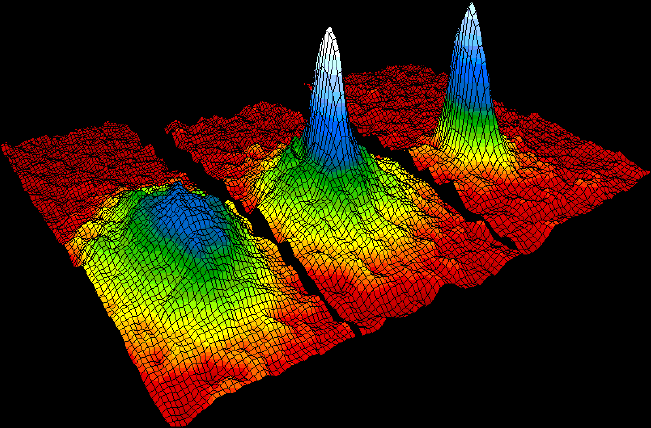
\includegraphics[width=0.6\linewidth]{fig/iconica.png}
\caption{Figura icônica da distribuição de velocidades do condensado de Bose-Einstein composto de átomos de Rubídio presos em armadilha parabólica.}
\label{fig:iconica}
\end{figure}

\n\n

(c) A energia do estado fundamental é $E_0 = \frac{1}{2} \hbar (\omega_x + \omega_y + \omega_z)$. Na transição para o condensado temos que $T \to T_c$, $\mu \to E_0$ e que $N_0 \to 0$ (número $N_0$ de partículas no estado fundamental só começa a ser macroscópico para $T < T_c$), de maneira que na transição temos
$$
N = \sum_{n_x, n_y, n_z} \frac{1}{e^{\beta(E_{n_x,n_y,n_z} - E_0)} - 1} =
\int_{-\infty}^{\infty} \int_{-\infty}^{\infty} \int_{-\infty}^{\infty}
\frac{\dd{n_x} \dd{n_y} \dd{n_z}}{e^{\frac{\hbar}{k_B T_c}(\omega_x n_x + \omega_y n_y + \omega_z n_z)} - 1}.
$$

Jogando essa integral no Mathematica, ele demora um pouco mas retorna
$$
N = \frac{\zeta(3)}{\omega_x \omega_y \omega_z} \, \qty(\frac{k_B T_c}{\hbar})^3 \implies
T_c = \frac{\hbar}{k_B} \qty(\frac{N \omega_x \omega_y \omega_z}{\zeta(3)})^{1/3}.
$$

Agora, no caso $T < T_c$ temos que a ocupação no estado fundamental é macroscópica ($N_0 > 0$). A ocupação nos estados excitados é
$$
N - N_0 = N_{E > E_0} = \int_{-\infty}^{\infty} \int_{-\infty}^{\infty} \int_{-\infty}^{\infty}
\frac{\dd{n_x} \dd{n_y} \dd{n_z}}{e^{\frac{\hbar}{k_B T}(\omega_x n_x + \omega_y n_y + \omega_z n_z)} - 1} =
\frac{\zeta(3)}{\omega_x \omega_y \omega_z} \, \qty(\frac{k_B T}{\hbar})^3 \implies
$$
$$
1 - \frac{N_0}{N} = \frac{\zeta(3)}{N \omega_x \omega_y \omega_z} \qty(\frac{k_B}{\hbar})^3 T^3 = \qty(\frac{T}{T_c})^3
\implies \boxed{ \frac{N_0}{N} = 1 - \qty(\frac{T}{T_c})^3. }
$$

\n

Na Seção 3.2 do artigo \cite{courteille2001} é possível encontrar a descrição do experimento de Cornell e Wieman para os átomos de Rubídio. Na subseção 3.2.1 temos o valor de frequência $\omega_{\text{TOP}} = 2\pi \times 7.5 \unit{kHz}$ e é dito que à temperatura $T = 90 \unit{\mu K}$ o condensado consistia de $4 \times 10^6$ átomos. Estimando o número de átomos, nós obtemos
$$
N = \zeta(3) \, \qty(\frac{k_B T}{\omega_{\text{TOP}} \hbar})^3 = 2 \times 10^7,
$$
que está quase na mesma ordem de grandeza dos $4 \times 10^6$ átomos, sendo superestimado por um fator $3$.


%%-----
%% Referências bibliográficas
%%-----
\addcontentsline{toc}{chapter}{\bibname}
%\bibliographystyle{abntex2-num}
\bibliography{citations}
\bibliographystyle{ieeetr}




\pagebreak

\section*{6) Paramagnetismo de Pauli}

(a) No limite de campo magnético $h \to 0$, temos que o potencial químico $\mu$ não se altera significativamente, $\mu(h) \approx \mu(h = 0) = \mu$.

Metade dos elétrons tem spin up $+1/2$ e a outra metade tem spin down $-1/2$. Devido ao campo magnético, ocorre um splitting nas energias. Os elétrons de spin up ficam com uma energia $\eps \to \eps - \mu_0 \mu_B h$ e os de spin down com $\eps \to \eps + \mu_0 \mu_B h$. Com essas considerações, temos
$$
N_+ = n_+ V = \frac{1}{2} \int n(E) D(E - \mu_0 \mu_B h) \dd{E} \e
N_- = n_- V = \frac{1}{2} \int n(E) D(E + \mu_0 \mu_B h) \dd{E},
$$
de maneira que $h = 0 \implies N_+ + N_- = \int n(E) D(E) \dd{E} = N$ (recuperamos o caso particular). A magnetização $m$ é então dada por
$$
m = - \mu_B (n_+ - n_-) =
\frac{\mu_B}{2V} \int n(E) \Big[ D(E + \mu_B h) - D(E - \mu_B h) \Big] \dd{E},
$$
mas como $h \to 0$, temos $D(E + \mu_0 \mu_B h) - D(E - \mu_0 \mu_B h) \approx 2 \mu_0 \mu_B h \, D'(E)$. Integrando por partes:
\begin{equation} \label{eq:magnetization}
m = \frac{\mu_0 \mu_B^2 h}{V} \int_{-\infty}^{\infty} n(E) D'(E) \dd{E}
\end{equation}
$$
= \frac{\mu_0 \mu_B^2 h}{V} \qty(\eval{n(E) D(E)}_{-\infty}^{\infty} - \int D(E) n'(E) \dd{E} ).
$$
Mas $D(\pm\infty) = 0$, portanto
$$
m = \frac{\mu_0 \mu_B^2 h}{V} \int D(E) \qty(- \pdv{n}{E}) \dd{E} \implies
\boxed{ \chi = \pdv{m}{h} = \frac{\mu_0 \mu_B^2}{V} \int D(E) \qty(- \pdv{n(E)}{E}) \dd{E}. }
$$

\n\n

(b) Para $T \to 0$, temos que $n(E) \to \theta_H(E_F-E)$ e usando a equação \ref{eq:magnetization}:
$$
m = \frac{\mu_0 \mu_B^2 h}{V} \int_{-\infty}^{\infty} n(E) D'(E) \dd{E} =
\frac{\mu_0 \mu_B^2 h}{V} \int_{-\infty}^{E_F} D'(E) \dd{E} =
\frac{\mu_0 \mu_B^2 h}{V} \qty[ D(E_F) - \cancelto{0}{D(-\infty)} ]
$$
$$
\implies \boxed{ \chi(T\to 0) = \pdv{m}{h} = \mu_0 \mu_B^2 \rho(E_F), }
$$
onde definimos $\rho(E) = D(E) / V$ como a densidade de estados por volume.

\n\n

(c) Para $T \to \infty$ ($\beta = \frac{1}{k_B T} \to 0$), podemos aproximar $n(E) \approx e^{-\beta(E - \mu)}$ (a distribuição de Fermi-Dirac tende à distribuição de Boltzmann em altas temperaturas) de maneira que $\pdv{n(E)}{E} \approx -\beta n(E)$. Portanto
$$
\chi(T \to \infty) = \frac{\mu_0\mu_B^2}{V} \int D(E) \qty(- \pdv{n(E)}{E}) \dd{E} \approx
\frac{\mu_0\mu_B^2}{V} \beta \underbrace{\int n(E) D(E) \dd{E}}_{N} \implies
$$
$$
\boxed{ \chi(T\to\infty) = \frac{N}{V} \, \frac{\mu_0 \mu_B^2}{k_B T}. }
$$



\end{document}
